Tiling the plane refers to covering the infinite flat surface of Euclidean geometry with repeated, gapless copies of one or more shapes. The problem is deceptively simple: given a shape, can it tile the plane? If so, does it do so uniquely, periodically, or in multiple distinct ways? In mathematics, tilings are not decorative but structural — they model how local adjacency rules propagate to infinite configurations. The arrangement must leave no gaps or overlaps and must cover the entire plane. These criteria make tiling an ideal setting to study how geometric structure interacts with combinatorial possibility, especially when infinite outcomes emerge from finite building blocks.

Classical tilings exhibit periodicity. That is, a finite patch of tiles can be shifted — translated — along certain vectors to cover the entire plane without change. This is the case for squares, equilateral triangles, and regular hexagons, all of which tile the plane in grid-like or honeycomb arrangements. The periodicity implies symmetry: the whole tiling looks the same from multiple viewpoints. Once a unit cell is known, the rest of the pattern follows. This repetition reflects the symmetry group of the tiling, which includes discrete translations and, often, rotations or reflections.

But not all tilings are periodic. Some are random or disordered, with tiles placed without a governing rule. Between these extremes lies a third category: aperiodic tilings. These are infinite tilings that never repeat, yet are constructed deterministically. They do not allow any nontrivial translation symmetry. Aperiodicity is not a lack of structure — it is a kind of order that defies repetition. In an aperiodic tiling, every finite patch occurs again and again throughout the plane, but never in a way that matches under translation. This intermediate form of order became a central question in mathematical tiling theory during the twentieth century.

A milestone came with the Penrose tiles: two simple shapes that, when used together with matching rules, could tile the plane only aperiodically. Their discovery provided the first explicit example of enforced aperiodicity in Euclidean space. The Penrose tilings exhibit hierarchical structure, rotational symmetries, and local rules that guarantee non-repetition globally. They also spurred new directions in mathematical logic, such as the undecidability of the domino problem, which asks whether a given set of tiles can tile the plane at all. But Penrose’s construction still relied on multiple tiles and decorations, raising a more restrictive question.

In 2023, a breakthrough resolved that question. A single 13-sided polygon, now known as the “hat,” was shown to tile the plane only aperiodically. Unlike previous examples, the hat requires neither additional markings nor complex matching rules. It is an ordinary polygon, unmarked and connected, yet it forces non-periodicity through geometry alone. The tiling requires both the tile and its mirror image, but nothing more. This monotile construction — the first of its kind — solved the so-called “Einstein problem” (named not after Albert Einstein but from the German \emph{ein Stein}, meaning “one tile”).

The hat enforces aperiodicity through the way its angles and edges constrain neighboring placements. When one tile is placed, the position and orientation of its neighbors are determined in such a way that no larger periodic patch can form. Though there is no explicit matching rule, the edge shapes themselves act as geometric constraints, preventing global repetition. This behavior is not stochastic: the rules are deterministic, and every valid tiling constructed from hats follows the same non-periodic principles.

This non-periodic structure is not chaotic. It satisfies a property called local isomorphism: every finite arrangement of tiles that appears anywhere in the tiling will appear again, infinitely often, but always at different locations and orientations. The tiling is thus filled with recurrence without translation. This balances two opposing tendencies — non-repetition on the global scale and determinism on the local one. It also implies that although no two regions of the tiling are exactly alike, they are compositionally similar in distribution.

The structure of the hat tiling is recursive. Tiles cluster into larger composite units — called “metatiles” — that mimic the form of the original. These metatiles then cluster into higher-order units in the same manner, forming a hierarchy of inflated self-similarity. Each level of the structure is built from the last by a fixed set of geometric rules, but the process never yields a lattice or periodic arrangement. This hierarchical self-assembly is one of the signatures of enforced aperiodicity in geometric tilings.

The implications of the hat tile reach beyond geometry. In materials science, aperiodic tilings model quasicrystals — atomic structures that lack translational symmetry but still produce sharp diffraction patterns. Such patterns indicate long-range order, even in the absence of repetition. The hat provides a new, purely geometric example of this phenomenon, offering abstract insight into the kinds of symmetries and constraints that physical matter can exhibit at the atomic scale.

From a mathematical perspective, the hat solves a long-standing open problem: whether a single, connected, unmarked tile could tile the plane only aperiodically. Previous constructions used markings, multiple shapes, or disconnected pieces. The hat showed that geometry alone could enforce the non-repetition constraint. It establishes the existence of a monotile — a single shape with no extra information — that forces infinite, non-repeating structure.

The discovery process itself is notable. David Smith, a retired printer and amateur tiling enthusiast, first noticed the tile’s behavior through hands-on experimentation. He shared it with researchers Craig Kaplan, Joseph Myers, and Chaim Goodman-Strauss, who formalized the result and constructed rigorous proofs. Their work combined visual intuition, algorithmic exploration, and mathematical formalism — demonstrating that significant advances in mathematics can still begin from curiosity and empirical play.

The hat tiling captures a central principle in mathematics: local rules can determine global behavior. From simple adjacency constraints, an entire infinite structure arises — deterministic, non-repeating, and deeply ordered.
\clearpage

\begin{commentary}[Commentary: Amateur Insight and Formal Machinery]
The hat tile was discovered not by formal derivation but by direct experimentation — David Smith observed its non-repeating behavior through hands-on manipulation. This empirical observation was later developed into a full mathematical result through collaboration with experts in geometry and substitution theory. The Spectre emerged from this joint effort, combining computational enumeration, combinatorial reduction, and formal inflation proofs. The case illustrates how mathematical insight can originate outside institutional settings and be sharpened into theorem by precise structural tools. Discovery here was stabilized through interaction between intuition and method.
\end{commentary}

\clearpage

\vspace{1em}
\begin{figure}[H]
\centering
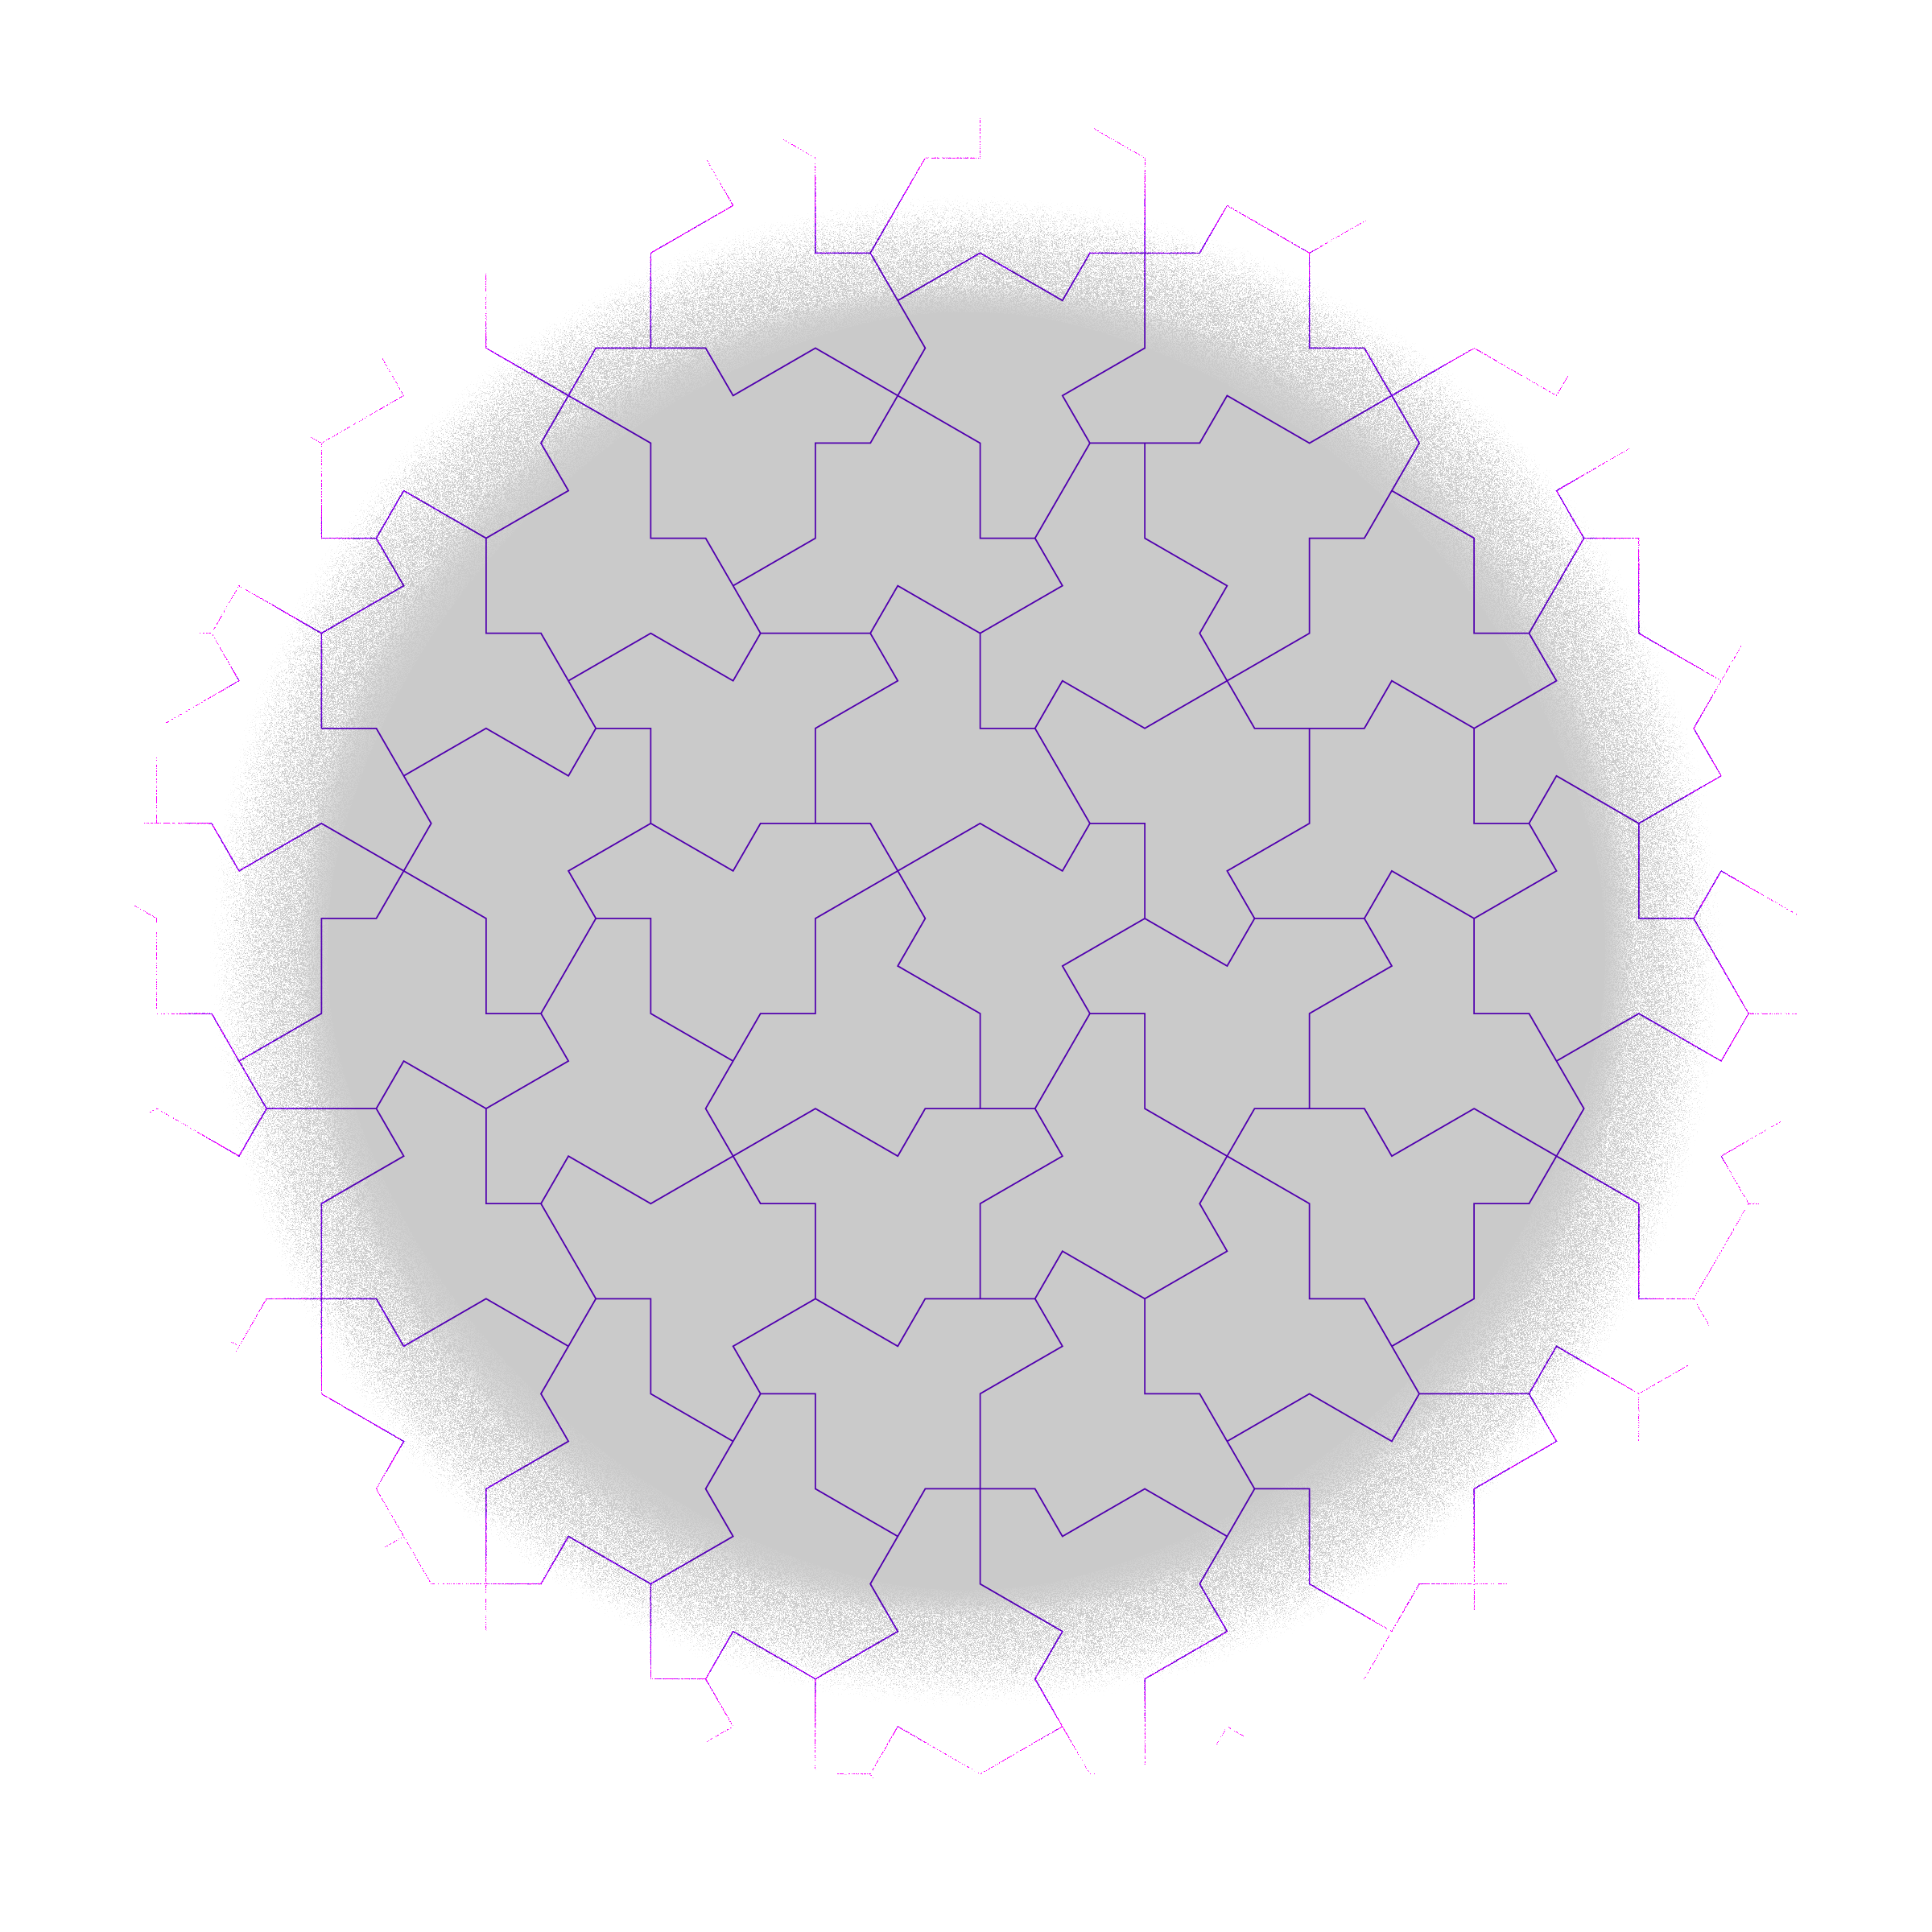
\includegraphics[width=0.8\linewidth]{29_HatMonotile/Aperiodic tile - puzzle.png}
\end{figure}

\clearpage
